\ifx\isEmbedded\undefined

\documentclass[12pt]{report}
	
% FONT RELATED
%\usepackage{times} %Move to times font
\usepackage[labelfont=bf,textfont=it]{caption}
\usepackage[utf8]{inputenc}

% LINKS, PAGE OF CONTENT, REF AND CROSS-REF, HEADERS/FOOTERS
\usepackage[hidelinks]{hyperref}
\usepackage{fancyhdr}
\usepackage{acronym}

% FIGURES, GRAPHICS, TABLES
\usepackage{graphicx}
\usepackage{parskip}
%\usepackage{subfigure}
\usepackage{subfig}
\usepackage{wrapfig}
\usepackage{subfloat}

% COLOURS, TEXT AND FORMATTING
\usepackage{array}
\usepackage{color}
\usepackage{setspace}
\usepackage{longtable}
\usepackage{multirow}

% ADVANCED MATHS, PSEUDO-CODE
\usepackage{amsmath}
\usepackage{alltt}
\usepackage{amsfonts}

% BIBLIOGRAPHY
\usepackage[authoryear]{natbib}
\bibpunct{(}{)}{;}{a}{,}{,}

% USE IN DISSER:

\setlength\oddsidemargin{0.85cm}
\setlength\evensidemargin{0.85cm}

\setlength\textheight{21.0cm}
\setlength\textwidth{15.0cm}

% indent at each new paragrapg
\setlength\parindent{0.5cm}

\setlength\topmargin{-0.2in}
\renewcommand{\baselinestretch}{1.3}

%REPORT

%\setlength\oddsidemargin{1cm}
%\setlength\evensidemargin{0.3in}
%%\setlength\headsep{2.5in}
%
%\setlength\textheight{9.0in}
%\setlength\textwidth{5.5in}
%
%% indent at each new paragrapg
%\setlength\parindent{0.5cm}
%
%%\setlength{\parskip}{10.5ex}
%
%\setlength\topmargin{-0.2in}

%\newcommand{\HRule}{\rule{\linewidth}{0.5mm}}
\newcommand{\HRule}{\rule{\linewidth}{0.0mm}}

% Color definitions (RGB model)
\definecolor{ms-comment}{rgb}{0.1, 0.4, 0.1}
\definecolor{ms-question}{rgb}{0.4, 0.0, 0.0}
\definecolor{ms-new}{rgb}{0.2, 0.4, 0.8}


\graphicspath{{../img/}}
\begin{document}
\fi

\chapter{Application Design and Implementation}
\label{chap:application_design_implementation}

\section{Design}

The developed application based on this approach was designed employing the Object Oriented Paradigm, aiming for a scalable and flexible system. It counts with a master class called \emph{CrowdEngine} which is the heart of the application. The \emph{CrowdEngine} stores all the agents and makes use of different classes in charge of other functions. The abstract class \emph{CellPartition} divides the space for an efficient handling. Currently, there is an unique specialized \emph{CellPartition}, the \emph{QuadraticGridCP}, but a \emph{CubicGridCP} might be included. The abstract class \emph{PhysicsEngine} is the responsible of collisions and applying external physical forces such as gravity or friction. So far, there are two \emph{PhysicsEngine}: \emph{CylinderPE} and \emph{SpherePE}. Finally, we count with an auxiliar specialized \emph{Parser} class to load agents from .txt files called \emph{TXTParser}.

\begin{landscape}

\begin{figure}[!htb]
  \centering
  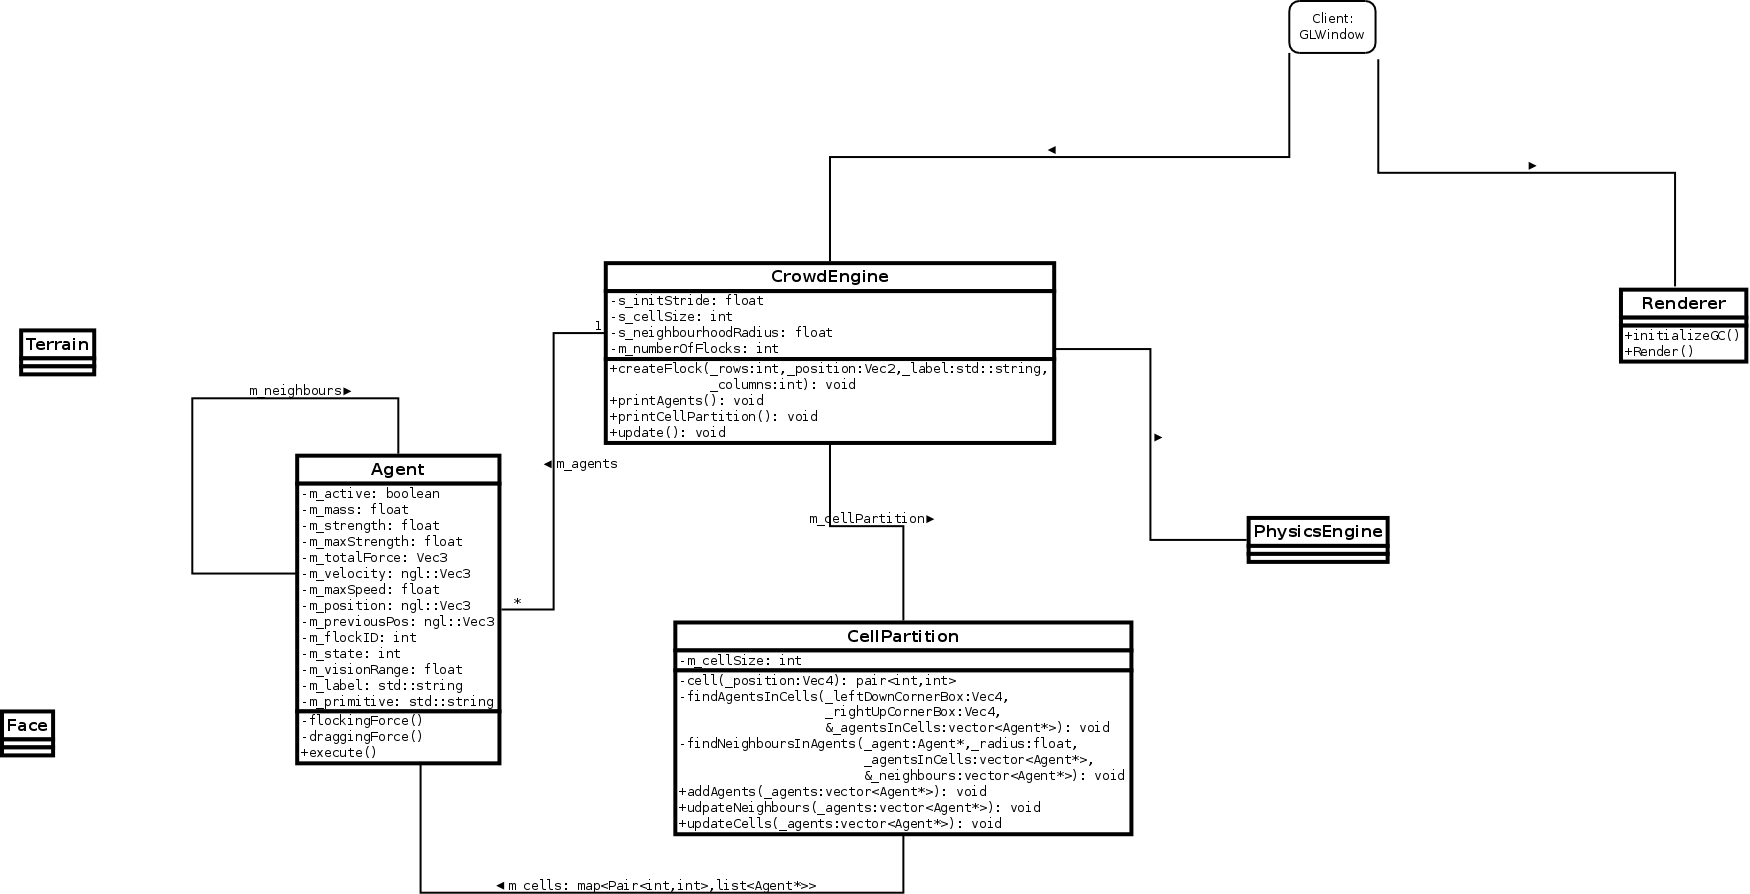
\includegraphics[scale=0.18]{classDiagram.eps}
  \caption{Class Diagram of the Application}
  \label{fig:classDiag}
\end{figure}

\end{landscape}

\section{Implementation}
The complete engine was implemented in the compiled language C++, employing the NGL library and some QT functions. Nevertheless, the brains of the agents were implemented in the scripted language Lua. In this way, it is not needed to recompile the whole application to load and run a new behaviour.

The LuaAPI was used in order to exchange data from the state of the application to the lua state which holds the brain-functions. Lua works using a stack, so when an agent is executed, it pushes on the stack all the information the brain needs and calls the brain-function. The brain pops the data and processes it, and then it will push onto the stack all the information relative to the new tick. \citep{lua}

One of the greatest advantages of this approach is the ability of script behaviours and test them in a quick and comfortable way. Due to this, infinite emergent behaviours can be created.

\ifx\isEmbedded\undefined
% References
\addcontentsline{toc}{chapter}{References}
\bibliographystyle{../ref/harvard}
\bibliography{../ref/master}
\pagebreak
\end{document}
\fi